%%%%%%%%%%%%%%%%%%%%%%%%%%%%%%%
% CHAPTER 4: EXPLORATORY STUDY
%%%%%%%%%%%%%%%%%%%%%%%%%%%%%%%
% METHOD
%%%%%%%%%%%%%%%%%%%%%%%%%%%%%%%%%%%%%%%%%%%%%%%%
%%%%%%%%%%%%%%%%%%%%%%%%%%%%%%%%%%%%%%%%%%%%%%%%
\newpage
\section{Method}
\label{exp-study:method}
% \textbf{Section~\ref{exp-study:method}}
%%%%%%%%%%%%%%%%%%%%%%%%%%%%%%%%%%%%%%%%%%%%%%%%
%%%%%%%%%%%%%%%%%%%%%%%%%%%%%%%%%%%%%%%%%%%%%%%%
% TOPLACE
% EXPAND: a simple criteria, definition of ``active''}. 
% METH Note quick and dirty, subjective analysis limitations.  Should be interpreted as indicative rather than conclusive.}
%%%%%%%%%%%%%%%%%%%%%%%%%%%%%%%%%%%%%%%%%%%%%%%%%%%%%%%%%%%%%%%%%%%%%%%%%%%%%%%%%%%%%%%%%%%%%%%%

%%%%%%%%%%%%%%%%%%%%%%%
% intro and structure
%%%%%%%%%%%%%%%%%%%%%%%
This section describes the methodology employed in the study.  \textbf{Section~\ref{exp-study:method-choice}} justifies the employment of semi-structured interviews, and \textbf{Section~\ref{exp-study:user-selection}} discusses the selection of participants.
\textbf{Section~\ref{exp-study:interview-process}} then outlines the interview structure and details the privacy-related precautions that were taken whilst working with personal data.  
%%%%%%%%%%%%%%%%%%%%%%%%%%%
% AND onto data analysis
%%%%%%%%%%%%%%%%%%%%%%%%%%%
% \textbf{Section~\ref{exp-study:ethics}} 
%Three novel analytical techniques are proposed by the author in the chapter, and are discussed in the final three sections. 
\textbf{Section~\ref{exp-study:data-analysis}} details data collection and provides an overview of data analysis, including the content analysis of the interview data.  This analysis focused on comparing the nature of PIM between the three tools in terms of the four sub-activities identified in \textbf{Chapter~\ref{chapter:bg}}.

The next three sections focus on the analysis of organizing behaviour.
% The next three sections detail the three novel techniques proposed by the author.
% ORG STRATGY COMPARISON
Firstly, \textbf{Section~\ref{exp-study:cross-tool-profiling}} discusses the comparison of organizing strategies between the three tools.
% ORG DIM COMPARISON
\textbf{Section~\ref{exp-study:folder-analysis-orgdim}} describes the analysis of folder structures in terms of \textit{organizational dimensions}, the types of concept on which folder names were based. % Firstly, \textbf{Section~\ref{exp-study:folder-analysis-orgdim}} details the analysis of folder structures in terms of \textit{organizational dimensions}. 
% FOLDER OVERLAP INVESTIGATION
Lastly, \textbf{Section~\ref{exp-study:analysis-folder-overlap}} reports the investigation of folder overlap, the extent to which folders relating to the same activity appear in multiple PIM-tools. % Then \textbf{Section~\ref{exp-study:analysis-folder-overlap}} then details the analysis of \textit{folder overlap} between pairs of folder structures. 

\textbf{Figure~\ref{fig:exp-study:analysis-structure}} provides a diagrammatic summary of data analysis.

% %%%%%%%%%%%%%%%%%%%%%%%%%%%%%%%%%%%%%%%%%%%%
% FIGURE - STAGES OF DATA ANALYSIS
% %%%%%%%%%%%%%%%%%%%%%%%%%%%%%%%%%%%%%%%%%%%%
\begin{figure}[hbtp]
	\begin{center}
		\leavevmode
			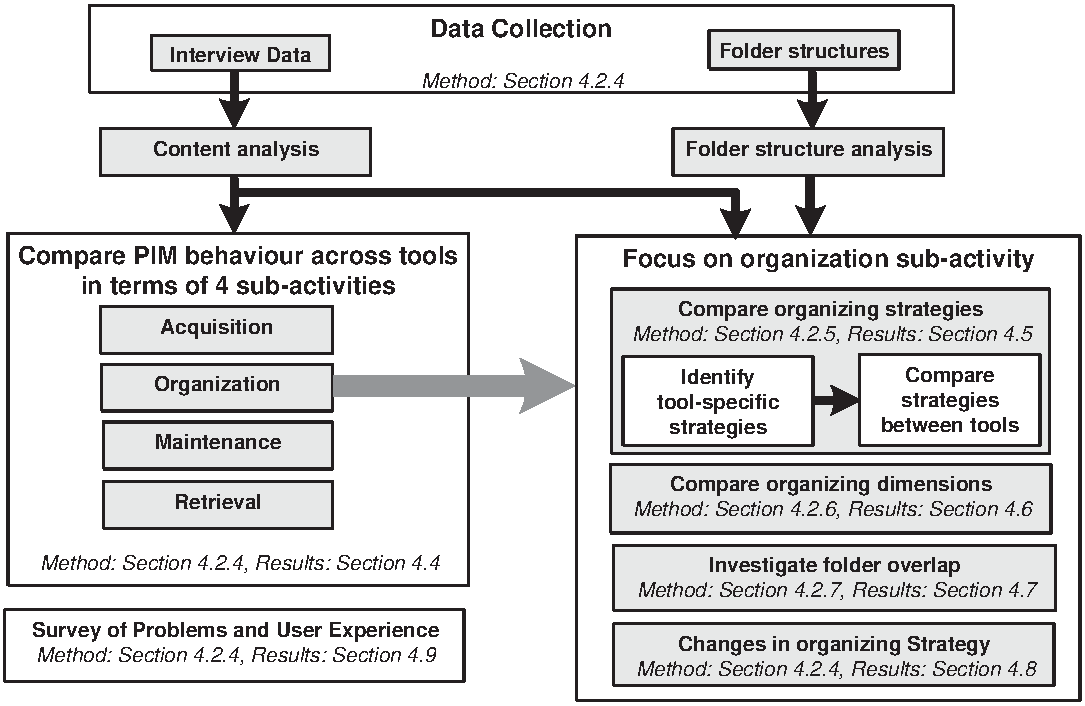
\includegraphics[height=10cm]{pictures/exp-study/analysis-structure.pdf}
		% \includegraphics[height=2in, width=.9 \textwidth]{pictures/exp-study-Overlaps.pdf}
	\end{center}
	\caption{Stages of data analysis}
	\label{fig:exp-study:analysis-structure}
\end{figure}



%%%%%%%%%%%%%%%%%%%%%%%%%%%%%%%%%%%%%%%%%%%%%%%%%%%%%%%%%%%%%%%%%%%%%%%%%%%%%%%%%%%%%%%%%%%%%%%%
%%%%%%%%%%%%%%%%%%%%%%%%%%%%%%%%%%%%%%%%%%%%%%%%%%%%%%%%%%%%%%%%%%%%%%%%%%%%%%%%%%%%%%%%%%%%%%%%
%%%%%%%%%%%%%%%%%%%%%%%%%%%%%%%%%%%%%%%%%%%%%%%%%%%%%%%%%%%%%%%%%%%%%%%%%%%%%%%%%%%%%%%%%%%%%%%%
%%%%%%%%%%%%%%%%%%%%%%%%%%%%%%%%%%%%%%%%%%%%%%%%%%%%%%%%%%%%%%%%%%%%%%%%%%%%%%%%%%%%%%%%%%%%%%%%

%%%%%%%%%%%%%%%%%%%%%%%%%%%%%
\subsection{Choice of Methodology}
\label{exp-study:method-choice}
% SECTION NOTES
% Inspired by the ethnographic method
% Interest: natural setting, investigate/explain phenomena in situ
% Can this be made more convincing?
% Wording: supporters of X claim
%%%%%%%%%%%%%%%%%%%%%%%%%%%%%%
A semi-structured interview methodology was selected, in which a core framework of questions forms the basis for the interviews. In addition, when time permits, the researcher can pursue diversions to related topics as they arise, giving the flexibility to elicit feedback on unexpected, yet relevant issues. This choice is justified for the following reasons. A key aim of the study was to investigate real-world PIM behaviour in a natural setting.  Semi-structured interviews are a standard HCI research methodology for investigating complex computer-based activities~\citep{Robson:01}.  Additionally, semi-structured interviews have been successfully employed in a number of previous studies of PIM, e.g. ~\citep{Whittaker-email:96}.  
 % The interview framework employed in this study is presented in \textbf{Section~\ref{exp-study:interview-process}}.
% Interview flexibility in this manner has proved to be successful in eliciting feedback on unexpected, yet relevant issues in HCI.

%%%%%%%%%%%%%%%%%%%%%%%%%%%%%%%%%%%%%%%%%%%%%%%%%%%%%%%%%%%%%%%%%%%%%%%%%%%%%%%%%%%%%%%%%%%%%%%%
%%%%%%%%%%%%%%%%%%%%%%%%%%%%%%%%%%%%%%%%%%%%%%%%%%%%%%%%%%%%%%%%%%%%%%%%%%%%%%%%%%%%%%%%%%%%%%%%
%%%%%%%%%%%%%%%%%%%%%%%%%%%%%%%%%%%%%%%%%%%%%%%%%%%%%%%%%%%%%%%%%%%%%%%%%%%%%%%%%%%%%%%%%%%%%%%%
%%%%%%%%%%%%%%%%%%%%%%%%%%%%%%%%%%%%%%%%%%%%%%%%%%%%%%%%%%%%%%%%%%%%%%%%%%%%%%%%%%%%%%%%%%%%%%%%

%%%%%%%%%%%%%%%%%%%%%%%%%%%%%%%%
\subsection{Participants}
\label{exp-study:user-selection}
%%%%%%%%%%%%%%%%%%%%%%%%%%%%%%%%
Twenty-five participants took part in the study.  An overview of their details is presented in \textbf{Table~\ref{table:exp-study:user_summary}}.  All participants had at least 5 years of general computing experience, and had used their current operating system for at least one year (19 used MS-Windows, 4 used MacOS, and 2 used Linux).  Of the 25 participants, 7 were female, and 18 were male.  The average age was 37 (ranging from 21 to 60).  The majority (23) were recruited from the academic establishments where the author was pursuing his research programme.
% from the universities where the author carried out his research or visited during his research (Imperial College London, University College London, Waikato University in New Zealand, and the University of Colorado at Boulder, USA).
Roles included researchers (12), students (10), and support staff (1). The final 2 were non-academic: one was a manager for a telecommunications company, and one was unemployed. Participants did not receive any incentive to take part, financial or otherwise. 

%%%%%%%%%%%%%%%%%%%%%%%%%%%%%%%%%%%%%%%%%%%%%%%%%%%%%%%
% TABLE: exploratory study participants
%%%%%%%%%%%%%%%%%%%%%%%%%%%%%%%%%%%%%%%%%%%%%%%%%%%%%%%
\begin{table}[hbt]
\begin{center}
\begin{footnotesize}
\setlength{\extrarowheight}{2pt}
%\begin{tabular}{|p{2.5cm}|p{3.5cm}|p{3.5cm}|p{3.5cm}|}
%	& {\bf Document File} & {\bf Email} &  {\bf Web} \\
% Table generated by Excel2LaTeX from sheet 'EXPLORATORY STUDY PARTICIPANTS'
\begin{tabular}{|c|c|c|c|c|c|}
\hline
    {\bf Participant} &  {\bf Age} &  {\bf Sex} & {\bf Job Role} & {\bf Location} & {\bf Operating System} \\
\hline
         P1 &      35-40 &          M &   Academic &         UK & Windows 2000 \\
\hline
         P2 &      20-25 &          M &    Student &         UK & Windows 2000 \\
\hline
         P3 &      25-30 &          M &    Student &         UK & Windows 2000 \\
\hline
         P4 &      20-25 &          F &    Student &         UK & Windows 2000 \\
\hline
         P5 &      25-30 &          M &    Student &         UK & Windows 98 \\
\hline
         P6 &        60+ &          M &   Academic &         UK &    MacOS 8 \\
\hline
         P7 &      25-30 &          M &    Student &         UK & Windows NT4 \\
\hline
         P8 &      25-30 &          M &    Student &         UK & Windows NT4 \\
\hline
         P9 &      45-50 &          F &   Academic &         NZ &     Macos8 \\
\hline
        P10 &      45-50 &          M &   Academic &         NZ & Windows NT4 \\
\hline
        P11 &      30-35 &          F &   Academic &         NZ & Windows NT4 \\
\hline
        P12 &      25-30 &          M &   Academic &         NZ &      Linux \\
\hline
        P13 &      50-55 &          M &   Academic &         NZ &    MacOS 9 \\
\hline
        P14 &      35-40 &          M &   Academic &         NZ & Windows 2000 \\
\hline
        P15 &      35-40 &          M &   Academic &         NZ & Windows NT4 \\
\hline
        P16 &      40-45 &          M & Technical Support &         NZ &    MacOS X \\
\hline
        P17 &      30-35 &          F &    Student &         NZ & Windows NT4 \\
\hline
        P18 &      25-30 &          M &    Student &         NZ &      Linux \\
\hline
        P19 &      35-40 &          M &   Academic &         NZ & Windows 2000 \\
\hline
        P20 &      30-35 &          M &    Student &        USA & Windows 2000 \\
\hline
        P21 &      30-35 &          F &    Student &        USA & Windows 98 \\
\hline
        P22 &      40-45 &          F &   Academic &         UK & Windows 98 \\
\hline
        P23 &      30-35 &          M &   Academic &         UK & Windows XP \\
\hline
        P24 &        60+ &          M & Unemployed &         UK & Windows 98 \\
\hline
        P25 &      40-45 &          F & Manager &         UK & Windows 2000 \\
\hline
\end{tabular}  
\end{footnotesize}
\caption{Participants in the Exploratory Study}
\label{table:exp-study:user_summary}
\end{center}
\end{table}
\normalsize

%%%%%%%%%%%%%%%%%%%%%%%%%%%%%%%%%%%%%%%%%%%%%%%%%%%%%%%%%%%%%%%%%%%
%\subsection{Working with personal information: ethics and privacy}
%\label{exp-study:ethics}
%%%%%%%%%%%%%%%%%%%%%%%%%%%%%%%%%%%%%%%%%%%%%%%%%%%%%%%%%%%%%%%%%%%
People known to the author were intentionally invited to participate due to concerns regarding the privacy issues associated with the researcher invading strangers' personal space. % check this!
It was envisaged that such familiarity would establish a trust basis, leading to the ability to raise concerns that may arise at any time.  Participants' comments (see \textbf{Section~\ref{exp-study:results-overview}}) suggest this was a valid consideration. 

%%%%%%%%%%%%%%%%%%%%%%%%%%%%%%%%%%%%%%%%%%%%%%%%%%%
% Limitations in terms of statistical significance
%%%%%%%%%%%%%%%%%%%%%%%%%%%%%%%%%%%%%%%%%%%%%%%%%%%
It is acknowledged that the study participants are not a representative sample of the general population of users, and are thus not statistically significant.  However, it is argued that the set of participants matches the purposes of the study well: to establish a comprehensive picture of users' PIM practices.   The results should be interpreted as suggestive (i.e. directed at forming the basis for future research) rather than as providing conclusive findings.
% Note that all the participants were known to the researcher before their participation in the study.  This user sample raises a key methodological point: it may be argued that the selection of participants who were familiar with the researcher may cause experimental bias.
% The selection of users is defended as follows.

%%%%%%%%%%%%%%%%%%%%%%%%%%%%%%%%%%%%%%%%%%%%%%%%%%%%%%%%%%%%%%%%%%%%%%%%%%%%%%%%%%%%%%%%%%%%%%%%
%%%%%%%%%%%%%%%%%%%%%%%%%%%%%%%%%%%%%%%%%%%%%%%%%%%%%%%%%%%%%%%%%%%%%%%%%%%%%%%%%%%%%%%%%%%%%%%%
%%%%%%%%%%%%%%%%%%%%%%%%%%%%%%%%%%%%%%%%%%%%%%%%%%%%%%%%%%%%%%%%%%%%%%%%%%%%%%%%%%%%%%%%%%%%%%%%
%%%%%%%%%%%%%%%%%%%%%%%%%%%%%%%%%%%%%%%%%%%%%%%%%%%%%%%%%%%%%%%%%%%%%%%%%%%%%%%%%%%%%%%%%%%%%%%%

% \newpage
%%%%%%%%%%%%%%%%%%%%%%%%%%%%%%%%
\subsection{Interview Process}
\label{exp-study:interview-process}
%%%%%%%%%%%%%%%%%%%%%%%%%%%%%%%%
% The core framework of each semi-structured interview was as follows.
% Wording: structured field notes sheet
%%%%%%%%%%%%%%%%%%%%%%%%%%%%%%%%
This section provides an overview of the interview format. Complete experimental materials are included in \textbf{Appendix~\ref{chap:appendices-exploratory-study-material}}.

Each interview lasted about 90 minutes, and was carried out in the usual workplace of the interviewee where it was possible to view the participant's activity in context.

%%%%%%%%%%%%%%%%%%%%%%%%%%%%%%%%%
% PRIVACY - BEFORE
%%%%%%%%%%%%%%%%%%%%%%%%%%%%%%%%%
Due to the highly personal nature of PIM, a number of privacy-related precautions were employed.  People frequently feel a sense of guilt towards a messy workspace, whether physical~\citep{tm:83} or electronic~\citep{Bellotti:00}.  % A view held by many people is that a ``tidy'' workspace, where all items are filed away, is superior to a ``messy'' workspace (CITE). However this popular belief has been debated in the literature~\citep{Whittaker-paper:01}.}.
Therefore a primary concern in the study was to not cause the participants to feel uncomfortable. 
The participants were made aware of the nature of the study in advance so that they could take steps to hide anything that they did not want the researcher to see (e.g. confidential information, medical reports, love letters!). However, the participants were asked not to change their collections in any other way before the interview (e.g. tidying their inbox).  This proved to be judicious, e.g. P25: \textit{``So you know what I do now - I would have tidied it up if you'd let me''}. 

%%%%%%%%%%%%%%%%%%%%%%%%%%%%%%%%%
% PRIVACY - START
%%%%%%%%%%%%%%%%%%%%%%%%%%%%%%%%%
Before each interview, the researcher stated that the user's personal approach to managing information was not being evaluated in any way, and all participants signed a release form acknowledging that the data would be anonymised before analysis and publication.  % Participants were reminded that the study was not intended to be a critique of how they organized their workspace.  
Next, basic demographic information was collected (summarized in \textbf{Table~\ref{table:exp-study:user_summary}}), and participants were asked about the main production activities which drove their computer usage. A screenshot of each participant's desktop was also captured.


%%%%%%%%%%%%%%%%%%%%%%%%%%%%%%%%%%%%%%%%%%%%%%%%%%%%%%%%%%%%%%%%%%%%%%%%%%%%%%%%%%%%%%%
% \subsubsection{Guided tour of the document file, email and web bookmarks collections}
%%%%%%%%%%%%%%%%%%%%%%%%%%%%%%%%%%%%%%%%%%%%%%%%%%%%%%%%%%%%%%%%%%%%%%%%%%%%%%%%%%%%%%%

Interviews were centred on guided tours of the files, email and bookmarks that they collected on their main work computer.

The three collections were defined as follows:

\begin{itemize}

%%%%%%%%%%%%%%%%%%%%%%%%%%%%%%%%%%%%%%%%%%
% Definition of file collection
%%%%%%%%%%%%%%%%%%%%%%%%%%%%%%%%%%%%%%%%%%
\item The \textit{document file collection} was defined as the principal area of the file system used by an individual to manage their personal document files. For the purposes of the study, document files were defined as those files containing content such as text, image and music files -- as opposed to executable applications. Since files are often distributed across multiple locations in the file system, participants were asked to identify their primary collection of personal files. Operating systems typically provide a default area for this purpose, such as ``My Documents'' under MS-Windows, or the ``home directory'' under UNIX.  Areas of the file collection that contained source code, simulation data, saved web pages, temporary files and internet downloads were omitted from the interview to save time.  In these cases, only the root folder of each sub-structure was surveyed.  So for example, if a file folder, \texttt{Downloads}, contained a set of sub-folders for downloaded programs, only the top folder was considered in the study.  % Hierarchies often contained extensive sub-structures for source code, simulation data, backups and temporary files. Only the root folder of such sub-structures was included. So for example, if a file folder sub-tree, \texttt{simproj/set3/monday/run2}, contained simulation data, only the top folder \texttt{simproj} was included.


%%%%%%%%%%%%%%%%%%%%%%%%%%%%%%%%%%%%%%%%%%
% Definition of email collection
%%%%%%%%%%%%%%%%%%%%%%%%%%%%%%%%%%%%%%%%%%
\item The \textit{email collection} was defined as the collection of electronic messages stored in the participant's main email tool.  If the participant employed multiple email tools (e.g. MS-Outlook on the desktop, and web-based email such as Hotmail), they were asked to nominate their primary collection.

%%%%%%%%%%%%%%%%%%%%%%%%%%%%%%%%%%%%%%%%%%
% Definition of bookmarks collection
%%%%%%%%%%%%%%%%%%%%%%%%%%%%%%%%%%%%%%%%%%
\item The \textit{web bookmark collection} was defined as the set of ``links'' or ``Favorites'' stored by a participant in their main web browser.
% SEE BELOW: why certain areas of the hierarchy omitted from the interview

\end{itemize}

The use of desktop icons to manage files, email, or bookmarks was also covered.  Icons were considered to be an adjunct to the respective collection.  

At the start of each guided tour, a snapshot was recorded of any folders developed by the participant.  Participants were asked to go through the folders one by one, and talk about their usage. Notes were made of folders that were mentioned as being no longer in use (e.g. failed or duplicate folders).  Participants were also asked about the function of any items that were not filed in folders (i.e. those items at the root-level of the collection, or those managed on the desktop). 

%%%%%%%%%%%%%%%%%%%%%%%%%%%%%%%%%
% PRIVACY - DURING
%%%%%%%%%%%%%%%%%%%%%%%%%%%%%%%%%
Wherever possible during the study, additional procedural steps were taken to avoid privacy infringements. For instance the exposure of the content of specific items of information was avoided wherever possible. One simple yet effective technique was to maximize the folder-view window, thus obscuring the content of specific items.
% Participants were able to do this either before or during the guided tours of their files, email and bookmarks.

During the guided tour participants were asked about their PIM practices within each collection. In order to cover the various aspects of PIM, the interview structure was based on the four point conceptual framework outlined in \textbf{Chapter~\ref{chapter:bg}}: \textit{acquisition} of items, \textit{organization} of those items, \textit{maintenance} of the collection, and \textit{retrieval} of items from the collection.  Participants were also asked about any problems they encountered in each PIM-tool.  Note that due to time limitations, interviews sometimes failed to cover all the above aspects. % EXPAND ME
% Note: that guided tours were not always complete due to lack of time on the part of the interviewer


%%%%%%%%%%%%%%%%%%%%%%%%%%%%%%%%%%%%%%%%%%%%%%%%%%%%%%%%
% Need to add? consideration of each tool separately
%%%%%%%%%%%%%%%%%%%%%%%%%%%%%%%%%%%%%%%%%%%%%%%%%%%%%%%%
% Note that each collection was covered separately. Any references made by the participant in the context of one collection to the other collections were noted (for instance the mention of files managed as attachments within email messages). Participants were asked to comment about the presence of similar folders in the different collections}.

%%%%%%%%%%%%%%%%%%%%%%%%%%%%%%%%%%%%%%%%%%%%%%%%%%%%%%%%%		
% \item \textbf{Overview of the rest of the workspace}
%%%%%%%%%%%%%%%%%%%%%%%%%%%%%%%%%%%%%%%%%%%%%%%%%%%%%%%%%
If time allowed, other collections of personal information were surveyed including those managed in the primary digital workspace (e.g. contacts), on mobile devices (e.g. PDA devices), and in the physical workspace (e.g. piles of documents).
% Although this framework defined the core of each interview, when time allowed diversions to related topics were permitted (e.g. other PIM tools and digital devices).







%%%%%%%%%%%%%%%%%%%%%%%%%%%%%%%%%%%%%%%%%%%%%%%%%%%%%%%%%%%%%%%%%%%%%%%%%%%%%%%%%%%%%%%%%%%%%%%%
%%%%%%%%%%%%%%%%%%%%%%%%%%%%%%%%%%%%%%%%%%%%%%%%%%%%%%%%%%%%%%%%%%%%%%%%%%%%%%%%%%%%%%%%%%%%%%%%
%%%%%%%%%%%%%%%%%%%%%%%%%%%%%%%%%%%%%%%%%%%%%%%%%%%%%%%%%%%%%%%%%%%%%%%%%%%%%%%%%%%%%%%%%%%%%%%%
%%%%%%%%%%%%%%%%%%%%%%%%%%%%%%%%%%%%%%%%%%%%%%%%%%%%%%%%%%%%%%%%%%%%%%%%%%%%%%%%%%%%%%%%%%%%%%%%

%%%%%%%%%%%%%%%%%%%%%%%%%%%%%%%%%%%%%%%%%
% METHOD 1
\subsection{Data Collection and Analysis}
\label{exp-study:data-analysis}
%%%%%%%%%%%%%%%%%%%%%%%%%%%%%%%%%%%%%%%%%

In order to build up a rich picture of participants' PIM practices, both subjective and objective data were collected .  User comments were captured as notes taken during the interview, and annotated with observations made by the researcher. A sample of the collected data is shown in \textbf{Appendix~\ref{chap:appendices--study-data}} on page~\pageref{chap:appendices--study-data:exp-study}.
% i.e. no transcriptions
Objective data was captured in the form of graphical snapshots of the desktop, and of any folder structures developed in each collection.  The author also recorded the number of unfiled items in each collection (items located in the root folder or on the desktop).

% The rest of this section surveys the data analysis that was performed: (1) content analysis of the interview notes, and (2) analysis of the folder structures.

%%%%%%%%%%%%%%%%%%%%%%%%%%%%%%%%%%%%%%%%%%%%%%%%%%%
\subsubsection{Content Analysis of Interview Notes}
%%%%%%%%%%%%%%%%%%%%%%%%%%%%%%%%%%%%%%%%%%%%%%%%%%%
% If required, follow-up meetings were arranged to clarify particular points that were not clear from the data.
% Also nature of items, of the collection in general.}
% changes in PIM strategy.
% integration between the three collections.
%%%%%%%%%%%%%%%%%%%%
% Old Stuff on WTBU
%%%%%%%%%%%%%%%%%%%%
% This qualitative data was used to characterise how participants managed each type of particular information and is reported in \textbf{Section~\ref{exp-study:Results1-WTBU}}.
% \item Content analysis of interview notes in terms of Barreau's conceptual framework.
Content analysis was performed on the interview data to extract key themes relating to PIM.
The content analysis consisted of several passes through the interview notes. A first pass lead to the development of a coding scheme listing key themes such as strategies, problems, design suggestions, and changes in strategy over time. Comments were also extracted relating to integration between PIM-tools. % both existing integration and needs for improved integration
During subsequent passes, the coding scheme was used to mark up the data, and extended with any further issues that emerged.  Finally, the themes were clustered using the four PIM sub-activities from
\textbf{Chapter~\ref{chapter:bg}} (acquisition, organization, maintenance, and retrieval), and arranged in terms of frequency and importance. % Relevant quotes were extracted to illustrate user behaviour.

The comparison of typical behaviour between the tools in terms of the four PIM sub-activities is reported in \textbf{Section~\ref{exp-study:Results-comparison}}\footnote{Note that the objective data (in the form of the folder hierarchies) was focused on one PIM sub-activity: organizing.  The non-longitudinal nature of the study meant that information regarding the other PIM sub-activities (acquisition, maintenance and retrieval) was as reported by each user and subjective in nature.}.  Changes in organizing strategy, and findings related to PIM problems are reported in \textbf{Sections~\ref{exp-study:comparison-changes}} and \textbf{\ref{exp-study:comparison-problems}} respectively.

\textbf{Section~\ref{exp-study:cross-tool-profiling}} describes how the qualitative data also contributed towards the classification of participants' organizing strategies with respect to files, email and bookmarks.

%%%%%%%%%%%%%%%%%%%%%%%%%%%%%%%%%%%%%%%%%%%%%%%%%%%
\subsubsection{Analysis of Folder Hierarchies}
%%%%%%%%%%%%%%%%%%%%%%%%%%%%%%%%%%%%%%%%%%%%%%%%%%%
% The analysis of folder structures consisted of three steps.

The folder hierarchies were transcribed, and marked up with participant's comments as to the function and usage of specific folders. % NB: this is a great argument for longitudinal studies
% Data analysis consisted of the following stages, including two novel techniques developed by the author to analyse and compare the folder hierarchies:
%%%%%%%%%%%%%%%%%%%%%%%%%%
% ANALYSIS1: BASIC STATS
%%%%%%%%%%%%%%%%%%%%%%%%%%
% NOT CAPTURED CONSISTENTLY: number of failed/active folders,
% THINK: need to explain hierarchy depth? (e.g. in email)
Then, basic statistics were extracted from each hierarchy including number of folders, number of unfiled items, and hierarchy depth. These are reported under the organizing PIM sub-activity in \textbf{Section~\ref{exp-study:comparison-organization}}.  As noted above, any file folder sub-structures containing source code, simulation data, or downloaded programs were omitted.

The folder structures were then analysed using two novel techniques, developed by the author.
%%%%%%%%%%%%%%%%%%%%%%%%%%%%%%%%%%%%%%%%
% ANALYSIS 2: ORGANISATIONAL DIMENSIONS
%%%%%%%%%%%%%%%%%%%%%%%%%%%%%%%%%%%%%%%%
\textbf{Section~\ref{exp-study:folder-analysis-orgdim}} reports the analysis of the \textit{organizational dimensions} used to name folders (e.g. \textit{project}, \textit{contact}, \textit{place}). 
%%%%%%%%%%%%%%%%%%%%%%%%%%%%%%%
% ANALYSIS 3: FOLDER OVERLAP
%%%%%%%%%%%%%%%%%%%%%%%%%%%%%%%
\textbf{Section~\ref{exp-study:analysis-folder-overlap}} reports the investigation of \textit{folder overlap}.

%%%%%%%%%%%%%%%%%%%%%%%%%%%%%%%%%%%%%%%%%%%%%%%%%%%%%%%%%%%%%%%%%%%%%%%%%%%%%%%%%%%%%%%%%%%%%%%%
%%%%%%%%%%%%%%%%%%%%%%%%%%%%%%%%%%%%%%%%%%%%%%%%%%%%%%%%%%%%%%%%%%%%%%%%%%%%%%%%%%%%%%%%%%%%%%%%
%%%%%%%%%%%%%%%%%%%%%%%%%%%%%%%%%%%%%%%%%%%%%%%%%%%%%%%%%%%%%%%%%%%%%%%%%%%%%%%%%%%%%%%%%%%%%%%%
%%%%%%%%%%%%%%%%%%%%%%%%%%%%%%%%%%%%%%%%%%%%%%%%%%%%%%%%%%%%%%%%%%%%%%%%%%%%%%%%%%%%%%%%%%%%%%%%


%%%%%%%%%%%%%%%%%%%%%%%%%%%%%%%%%
% METHOD 2
%\subsection{Method: Comparing PIM Behaviour}
%\label{exp-study:behaviour-comparison}
%%%%%%%%%%%%%%%%%%%%%%%%%%%%%%%%%
%%%%%%%%%%%%%%%%%%%%%%%%%%%%%%%%%
%%%%%%%%%%%%%%%%%%%%%%%%%%%%%%%%%
% CONTENT1: Comparing the nature of PIM
%%%%%%%%%%%%%%%%%%%%%%%%%%%%%%%%%
% For each PIM sub-activity, typical behaviour was compared between the three PIM-tools, to investigate whether similar strategies were used to manage different types of information. Based on these tool-specific characterizations, the management of each type of information was compared at an abstract \textit{cross-user} level (generalized across all participants) to answer the question: \textit{Across participants in general, how does the management of the three types of information compare?}. These results are reported in \textbf{Section~\ref{exp-study:Results-comparison}}.


%%%%%%%%%%%%%%%%%%%%%%%%%%%%%%%%%%%%%%%%%%%%%%%%%%%%%%%%%%%%%%%%%%%%%%%%%%%%%%%%%%%%%%%%%%%%%%%%
%%%%%%%%%%%%%%%%%%%%%%%%%%%%%%%%%%%%%%%%%%%%%%%%%%%%%%%%%%%%%%%%%%%%%%%%%%%%%%%%%%%%%%%%%%%%%%%%
%%%%%%%%%%%%%%%%%%%%%%%%%%%%%%%%%%%%%%%%%%%%%%%%%%%%%%%%%%%%%%%%%%%%%%%%%%%%%%%%%%%%%%%%%%%%%%%%
%%%%%%%%%%%%%%%%%%%%%%%%%%%%%%%%%%%%%%%%%%%%%%%%%%%%%%%%%%%%%%%%%%%%%%%%%%%%%%%%%%%%%%%%%%%%%%%%

% \newpage
%%%%%%%%%%%%%%%%%%%%%%%%%%%%%%%%%
%%%%%%%%%%%%%%%%%%%%%%%%%%%%%%%%%
% METHOD 4
\newpage
\subsection{Method: Comparing Organizing Strategies}
\label{exp-study:cross-tool-profiling}
%%%%%%%%%%%%%%%%%%%%%%%%%%%%%%%%%
%%%%%%%%%%%%%%%%%%%%%%%%%%%%%%%%%
% \textbf{Section~\ref{exp-study:cross-tool-profiling}} details the cross-tool profiling of individuals' filing behaviour.

The analysis of organizing strategies consisted of two stages:
\begin{enumerate}
	\item Classifying each participants' strategies in each collection in turn.
	\item Comparing each participants' strategies between their three collections.
\end{enumerate}

%%%%%%%%%%%%%%%%%%%%%%%%%%%%%
% TOOL-SPECIFIC PROFILING
%%%%%%%%%%%%%%%%%%%%%%%%%%%%%
Firstly, organizing strategies were characterised for each participant in the 3 PIM-tools.
% \textbf{Section~\ref{exp-study:data-analysis}} describes the content analysis performed to identify the management strategies employed by participants in each of the three tools.
In each tool a classification scheme was devised by the author to categorize the participants based on their reported management strategies.  Previous classifications of organizing strategies that have been proposed in email~\citep{Whittaker-email:96} and for bookmarks~\citep{da:98} were used as a starting point in those two contexts.  Classifications were based on a combination of objective data (e.g. folder counts) and participants' comments.  Qualitative data was employed as it was not always straightforward to distinguish current strategies based on objective data alone.  For instance, a large folder count may suggest a user who files most information.  However, in many cases folders were abandoned.  Qualitative data was useful in indicating whther this was the case.
The three tool-specific classification schemes (for files, email, and bookmarks) are reported in \textbf{Sections~\ref{exp-study:Results-org-strategies-files}}, \textbf{\ref{exp-study:Results-org-strategies-email}}, and \textbf{\ref{exp-study:Results-org-strategies-bookmarks}}.

%%%%%%%%%%%%%%%%%%%%%%%%%%%%%%%%%
% CROSS-TOOL PROFILING
%%%%%%%%%%%%%%%%%%%%%%%%%%%%%%%%%
% Based on this within-tool analysis, the nature of PIM is compared between the three tools.
% The data relating to each PIM-tool was collated together across all participants. Then for each PIM-tool, the most common PIM strategies were identified, and a classification of user behaviour proposed.
% This analysis was aimed at characterizing the most common PIM practices -- observed across all participants -- regarding each type of information (technological format) in turn: files, email, and bookmarks. 
% WT/BU PERSPECTIVE: This analytical perspective is equivalent to that employed in previous tool-specific studies (see \textit{\textbf{Chapter~\ref{chapter:review}}}), and can be considered as an attempt to answer the question: \textit{Can PIM practices within particular collections be characterized across all study participants?} 
% By comparing the management of a particular type of information across multiple users, it is possible to classify the users in terms of the strategies used to manage files, email and bookmarks in turn.
% A particular focus was taken on the sub-activity of organization, and for each tool a classification of participants' reported filing behaviour is presented. 
The comparison stage was carried out to investigate whether individual participants employed consistent organizing strategies across their collections. The driving interest was to investigate whether participants who were relatively organized in files were also relatively organized in the other tools, and vice versa.  For each participant, a cross-tool profile was produced by collating the three tool-specific strategies from the previous stage.  Since the cross-tool profiling employed the tool-specific classifications, the method is discussed in detail in \textbf{Section~\ref{exp-study:Results-cross-tool-profiling}}, along with the results.
% This was performed to investigate whether individual participants employed consistent strategies across their collections (in terms of whether they reported devoting significant effort to organizing multiple types of information). 

%WE compared each participant's organizing strategies between the three collections to investigate the consistency of their organizing/filing behaviour.
% This approach goes beyond previous work by attempting to build up a \textit{cross-tool} profile of user behaviour.
Previous empirical studies have focused on individual usage of specific tools such as email. In contrast, this analysis attempts to go beyond previous work by constructing a cross-tool profile of behaviour to investigate how organizing practices vary between the collections for individual users.  % The \textit{cross-tool profiling} technique is described in more detail in \textbf{Section~\ref{exp-study:cross-tool-profiling}}.
% The previous analysis compared generalized behaviour between the tools.
% Rather than generalizing across all participants as in the previous stage, the aim was to focus on individuals. This analysis was directed at exploring similarities and differences between the three collections to investigate potential compatibility for integration and/or unification.





%%%%%%%%%%%%%%%%%%%%%%%%%%%%%%%%%%%%%%%%%%%%%%%%%%%%%%%%%%%%%%%%%%%%%%%%%%%%%%%%%%%%%%%%%%%%%%%%
%%%%%%%%%%%%%%%%%%%%%%%%%%%%%%%%%%%%%%%%%%%%%%%%%%%%%%%%%%%%%%%%%%%%%%%%%%%%%%%%%%%%%%%%%%%%%%%%
%%%%%%%%%%%%%%%%%%%%%%%%%%%%%%%%%%%%%%%%%%%%%%%%%%%%%%%%%%%%%%%%%%%%%%%%%%%%%%%%%%%%%%%%%%%%%%%%
%%%%%%%%%%%%%%%%%%%%%%%%%%%%%%%%%%%%%%%%%%%%%%%%%%%%%%%%%%%%%%%%%%%%%%%%%%%%%%%%%%%%%%%%%%%%%%%%

%%%%%%%%%%%%%%%%%%%%%%%%%%%%%%%%%
%%%%%%%%%%%%%%%%%%%%%%%%%%%%%%%%%
% METHOD 2
\subsection{Method: Analysis of Organizational Dimensions}
\label{exp-study:folder-analysis-orgdim}
%%%%%%%%%%%%%%%%%%%%%%%%%%%%%%%%%
%%%%%%%%%%%%%%%%%%%%%%%%%%%%%%%%%
% employed in the \textit{within-tool/between-users analysis} detailed below
% These results are reported along with the qualitative findings relating to folder organization in
% %  For example the email folder ``Eric'' is based on \textit{contact}.  This technique was used to compare the types of folders created in the three collections of personal information. The motivation and execution of this technique is discussed in more detail in .  % Results are reported in \textbf{Section~\ref{exp-study:Results-org-dims}}.
% including the most common organizational dimensions used to classify each type of information. 
%%%%%%%%
% INTRO
%%%%%%%%
% The technique was used to characterize the types of folders developed within each collection of personal information. 
% The term \textit{organizational dimension} is used in this thesis to mean type of concept on which a folder name is based.  
This section presents a technique developed by the author to analyse the \textit{organizational dimensions} present in a folder structure -- \textit{the types of concept on which folder names are based (e.g. project, place, contact)}.


% Firstly, the rationale behind the technique is discussed, followed by detail of its execution.
%%%%%%%%%%%%%%%%%%%%%%%%%%%%%%%%%%%%
\subsubsection{Motivation and Aim}
%%%%%%%%%%%%%%%%%%%%%%%%%%%%%%%%%%%%
%% ADD other terms for organizational dimension in the literature.
%% Common examples noted in the literature include events (e.g. ``Jill's wedding''), roles (e.g. ``Teaching'') and people (e.g. ``Brian'') (\textit{CITE}). 
The development of the technique was motivated on two counts.
Firstly, previous studies have noted the existence of particular types of folders. For instance, \citet{Ducheneaut:01} observed that most email folders were based on \textit{sender}, \textit{organization}, \textit{project}, or \textit{interest}.  They also observed that the relative proportions of folder types varied significantly between users.  Similar \textit{ad hoc} observations of common folder types have been used by designers as the design rationale for PIM-unification systems based on a dominant organizational dimension such as \textit{role}~\citep{Shneiderman:94} or \textit{project}~\citep{Kaptelinin:03}.  However, no systematic analysis of folder types has been performed to date.

Secondly, during the guided tours in this study, many participants referred to various organizational dimensions. % Commonly mentioned folder types included \textit{projects}, \textit{roles} and \textit{interests}.
For example, P22 summarized her file folders as follows: \textit{``They are organized by projects, activities and roles such as `PhD tutor'. Oh, and this is bad, I also have a `Papers' folder where I keep all the papers that I've written, authored or co-authored. And they're broken down by co-author, cos I'm usually a co-writer''}.  In this statement four organizational dimensions are cited: \textit{projects}, \textit{activities}, \textit{roles} and \textit{people}. % Such dimensions can be considered as a description of the types of concept on which folder names are based.

%%%%%%%
% Aims
%%%%%%%
%%%%%%%%%%%%%%%
% Implications
%%%%%%%%%%%%%%%

% As a first step WE were interested in generalizing our analysis of organizational dimensions across users: \textit{Are personal information collections of a particular technological format dominated by particular organizational dimensions? Are different types of information dominated by different sets of organizational dimensions?}
% My \textit{a priori} hypothesis, based on what WE had seen in the data was that users employ a wide variety of organisational dimensions to structure their collections of document files, email and web bookmarks.
The objective of this analysis was two-fold.
\begin{enumerate}
% (1) explore what types of organizational dimension appeared in each tool (\textit{Research question: what types of organizational dimension are meaningful for users when organizing a particular type of information?}), 
\item To characterise the most common organizational dimensions within each PIM-tool. 
% and then (2) (\textit{Research question: How do organizational dimensions vary between tools?}.
% this would indicate that the users require a high level of organisational flexibility. T  
\item To compare PIM-tools in terms of their most common organizational dimensions.
\end{enumerate}

%%%%%%%%%%%%%%%%%%%%%%%%%%%%%%%
% Relate to previous studies
%%%%%%%%%%%%%%%%%%%%%%%%%%%%%%%
%% Avoid repeating the literature review!
%%
%% Points to get in comparing my approach to Barreau etc.'s: In the style of Kwasnik and Barreau, this study is based on the subjects' own resources (\textit{ADD: unlike GD}). 
%
% \textit{Focus on folders-only (plus user description) versus general description of classification behaviour -- talking generally about handling items (not quite true, WE annotated folder lists with user comments). In contrast to all three previous studies, dimensional analysis is based directly on folder names (and the descriptions participants offered of those folder names offered during the guided tour. In the previous studies analysis was based on general descriptions of classificatory behaviour. The more direct approach was chosen because of the larger amount of material to be analysed (in terms of number of users and number of classification schemes compared to the above studies). }
The existence of a dominant dimension across all tools for a particular user may indicate an optimum subordinate dimension for unification.  In contrast, if a user employs a variety of dimensions across different collections, this would represent a possible barrier against unification, and suggest that basing organizational support on a single subordinate dimension such as \textit{role}~\citep{Shneiderman:94} would overly constrain that user.

This approach can be contrasted with earlier investigations of classification behaviour in physical document~\citep{kwas:91}, digital file~\citep{barreau:95}, and web bookmark collections~\citep{gd:01}. In this body of previous work, analysis was centred on participants' descriptions of their classificatory behaviour.  Here, analysis focused on folder names and the descriptions of those folder names offered by participants during the guided tour.  In addition, this study compares between three different PIM-tools.
% In her study of physical PIM, Kwasnik~\citep{kwas:91} identified a range of factors that influenced the classification included those based on attributes of the document content such as author and topic, and those based on document context such as importance and activity. A similar technique has been employed more recently in the electronic domain in studies of applied similar methods to the electronic domain, in their studies of files~\citep{barreau:95} and web bookmarks~\citep{gd:01}. 



%%%%%%%%%%%%%%%%%%%%%%
\subsubsection{Method}
%%%%%%%%%%%%%%%%%%%%%%

A coding scheme was developed representing the various organizational dimensions manifested in folder names.  The scheme was initially seeded based on proposed PIM-unification technologies that have been based on a subordinate organizational dimension: \textit{role} (defined as long-term user activity)~\citep{Shneiderman:94}, \textit{project} (defined as short-term user activity)~\citep{Kaptelinin:03}, \textit{time}~\citep{Gelernter:96a} and \textit{contact}~\citep{Whittaker-contactmap:02b}.
An iterative coding process was then applied to the folder structures. Each file, email and bookmark folder was coded with the most relevant organizational dimension. At the same time, the coding scheme was extended to include organizational dimensions that were not represented.  Eventually a list of seventeen organizational dimensions was finalized that classified all the folders generated by the participants. 
% CHECK NUMBER fourteen fourteen
% CHECK NUMBER fourteen fourteen
% CHECK NUMBER fourteen fourteen
% CHECK NUMBER fourteen fourteen% CHECK NUMBER fourteen fourteen% CHECK NUMBER fourteen fourteen
% CHECK NUMBER fourteen fourteen
% CHECK NUMBER fourteen fourteen% CHECK NUMBER fourteen fourteen
% CHECK NUMBER fourteen fourteen
The final coding scheme is shown in \textbf{Table~\ref{table:exp-study:dimensions}}, along with some example folders of each type. % Folders were also coded with the secondary dimensions based on comments made during the interviews: coding-related folder (\#), shared folder (+), failed (empty) folder (-), and duplicate folder (\%).

% %%%%%%%%%%%%%%%%%%%%%%%%%%%%%
% TABLE - CODING SCHEME FOR ORGDIMS
% %%%%%%%%%%%%%%%%%%%%%%%%%%%%%
\begin{table}[hbt]
\begin{center}
\begin{footnotesize}
\setlength{\extrarowheight}{2pt}
\begin{tabular}{|c|c|p{3cm}|p{3cm}|}
\hline
{\bf Organisational dimension} & {\bf Code} & {\bf Description} & {\bf Examples} \\
\hline
Project &          P & Short-term production activity & ``Experiment'', ``Agent code'' \\
\hline
Role &          R & Long-term production activity & ``Teaching'', ``Personal'' \\
\hline
Topic / Interest &          I & Subject matter of item & ``Banking'', ``Science Fiction'' \\
\hline
Contact &          C & individual or organisation & ``Rick'', ``ACM'' \\
\hline
Time &          T &  & ``February'', ``tomorrow'' \\
\hline
General &          G &  & ``Stuff'', ``misc'' \\
\hline
Format &          F & Technological format of item & ``Excel sheets'', ``Word document'' \\
\hline
Class of document &          d & Type/class of item & ``Letters'', ``References'' \\
\hline
Workflow &          W &            &  ``Pending'' \\
\hline
Event &          E & Related to a particular occasion such as a meeting or conference &  ``CHI2000'' \\
\hline
Mailing list &          L &            & ``linux-users'' \\
\hline
Version control &          V &            & ``version1'', ``old'' \\
\hline
 Temporary &          t &            & ``temp'', ``tmp'' \\
\hline
Application &          A & Generated automatically by software & ``From ICQ'' \\
\hline
Backup &          B  &            & ``backup'', ``archive'' \\
\hline
Use &          U  &            & ``important'' \\
\hline
Geographic location &          G  &            & ``peckham'' \\
\hline
\end{tabular}  
\end{footnotesize}
\caption{Coding scheme of organizational dimensions}
\label{table:exp-study:dimensions}
\end{center}
\end{table}

Each folder was mapped to one dimension only.  \citet{jc:82} observed complex conventions for naming files.  Similarly complex folder-naming schemes were observed here, and in some cases folder labels were made up of several dimensions. For instance, \texttt{Personal-May} is made up of a combination of the \textit{role} and \textit{time} dimensions.  In such cases, only the first dimension was coded against the folder. %% CHECK

Hierarchies often contained extensive sub-structures for source code, simulation data, backups and temporary files. Only the root folder of such sub-structures was included. So for example, consider a file folder sub-structure, \texttt{simproj/set3/monday/run2}, containing simulation data. In this case, only the top folder \texttt{simproj} was included as a \textit{project} folder.

%%%%%%%%%%%%%%%%%%%%%%%%%%%%%%%%%%%%%%%%%%%
% DIFFICULTIES IN ASSIGNING FOLDER CODES
%%%%%%%%%%%%%%%%%%%%%%%%%%%%%%%%%%%%%%%%%%%
% \textit{Explain why this was not a problem!}.
Folder labels that were ambiguous in some way were confirmed with the subject when possible. Where this was not possible, a subjective coding decision was made by the researcher.  Assigning dimensions involved several challenges:

% However, in some cases, the meaning of particular folders was difficult to interpret. 
\begin{enumerate}

\item \textit{Deciphering abbreviated folder names} -- Some short-hand folder names were difficult to interpret, e.g. participant P24 had many minimal folder names such as \texttt{a2} and \texttt{fjk}.

\item \textit{Non-English folder names} -- Most participants used English to label folders.  However, since participants were drawn from a wide range of nationalities, several other languages were occasionally used to name folders, including Swedish, German, and Portuguese.  In such cases participants were asked for a translation.  % All were asked for translations during interviews where possible. 

\item \textit{Ambiguous folder-to-code mapping} -- In some cases, it was possible to map folder names to multiple codes.  For example, the folder \texttt{jobs} may be interpreted in three ways: (1) as a \textit{document class} (i.e. job adverts), (2) as a \textit{topic}, or (3) as a surname (\textit{contact}).  In the absence of a description from the participant, an estimation was made by the researcher.

% The author attempted to map folders to codes based on the participant's description.

% \item \textit{Multiple folder-to-code mappings} --  % \textbf{CHECK THIS}.

% \textbf{Add examples}.
\end{enumerate}		

%%%%%%%%%%%%%%%%%%%%%%%%%%%%%%
% Collate across all users
%%%%%%%%%%%%%%%%%%%%%%%%%%%%%%
For each PIM-tool, the most common organizational dimensions were identified by collating the coded data across all users.  The results of this analysis are reported in \textbf{Section~\ref{exp-study:Results-org-dims}}. This technique was also used in the subsequent investigation of folder overlap (see \textbf{Section~\ref{exp-study:analysis-folder-overlap}}). % The results of this analysis are reported in \textbf{Section~\ref{exp-study:Results-folder-overlap}}.


%%%%%%%%%%%%%%%%%%%%%%%%%%%%%%%%%%%%%%%%%%%%%%%%%%%%%%%%%%%%%%
% Limitations: only concerned with organizational metadata.
%%%%%%%%%%%%%%%%%%%%%%%%%%%%%%%%%%%%%%%%%%%%%%%%%%%%%%%%%%%%%%
% (\textit{ADD DEFINITION IN PIM-CF}).
%  No attention was paid to any implicit metadata that the users relied on when sorting information (e.g. \textit{subject} or \textit{date received} in email).
Several limitations to this analysis are acknowledged.  Firstly, the analysis is based on explicit structural metadata only -- other forms of organization was not encompassed (e.g. spatial grouping of icons on the desktop).  Secondly, some areas of the folder structures were omitted (e.g. temporary data). Finally, in the cases outlined above, coding may have been non-optimal.  Therefore the results should be taken as indicative only. However, it is argued that these limitations are acceptable considering the exploratory nature of the study.
% this maps well to the aim of the study: to get an overview comparison of how different types of information are managed.



%%%%%%%%%%%%%%%%%%%%%%%%%%%%%%%%%%%%%%%%%%%%%%%%%%%%%%%%%%%%%%%%%%%%%%%%%%%%%%%%%%%%%%%%%%%%%%%%
%%%%%%%%%%%%%%%%%%%%%%%%%%%%%%%%%%%%%%%%%%%%%%%%%%%%%%%%%%%%%%%%%%%%%%%%%%%%%%%%%%%%%%%%%%%%%%%%
%%%%%%%%%%%%%%%%%%%%%%%%%%%%%%%%%%%%%%%%%%%%%%%%%%%%%%%%%%%%%%%%%%%%%%%%%%%%%%%%%%%%%%%%%%%%%%%%
%%%%%%%%%%%%%%%%%%%%%%%%%%%%%%%%%%%%%%%%%%%%%%%%%%%%%%%%%%%%%%%%%%%%%%%%%%%%%%%%%%%%%%%%%%%%%%%%

% \newpage
%%%%%%%%%%%%%%%%%%%%%%%%%%%%%%%%%
%%%%%%%%%%%%%%%%%%%%%%%%%%%%%%%%%
% METHOD 3
\subsection{Method: Analysis of Folder overlap}
\label{exp-study:analysis-folder-overlap}
%%%%%%%%%%%%%%%%%%%%%%%%%%%%%%%%%
%%%%%%%%%%%%%%%%%%%%%%%%%%%%%%%%%

This section describes the second novel technique developed by the author to analyse personal folder structures. The technique is used for assessing the similarity of two collections of personal information in terms of \textit{folder overlap}: the extent to which folders referring to the same activity appear in multiple collections. % CHANGE

%%%%%%%%%%%%%%%%%%%%%%%%%%%%%%%%%%%%
\subsubsection{Motivation and Aim}
%%%%%%%%%%%%%%%%%%%%%%%%%%%%%%%%%%%%
The technique was motivated as follows. Firstly, previous studies have observed overlapping folders.  For example, \citet{Kaptelinin:03} notes that a user may manage and organize multiple types of information when working on a particular project.  He notes that a user working on a software project may author source code documents, receive emails and browse useful websites whilst carrying out the work -- and file them within identical folders in each tool. However, no systematic investigation of folder overlap across a set of users has been carried out.

Additionally, during the guided tours in this study, several participants commented on folders that had appeared in other collections. For a few participants, some folders overlapped between all three collections. For example, P14 had \texttt{Teaching}, \texttt{Research} and \texttt{Personal} folders in his file, email \textit{and} web bookmark hierarchies.  More commonly, there was a partial overlap which varied between the different pairs of collections, e.g. P13: \textit{``The email folders are fairly close to the file system, but with some differences. For example this folder contains correspondence-based information which does not make sense in the file system''}.  



The aim here was to go beyond previous work, and investigate the extent of folder overlap for each participant.  The author was interested in how folder overlap might be used as a measure of the compatibility of different personal classification schemes to be unified.  % Folder overlap may relate to activities that involve the organization of multiple types of information, and thus have the most to gain from increased integration.

%%%%%%%%%%%%%%%%%%%%%%
% MOVE TO RESULTS?
%%%%%%%%%%%%%%%%%%%%%%
% Such activities may have most to benefit from increased integration between PIM tools.  
% It was hypothesised that folder overlap may indicate that the different personal classification schemes tend to converge even when managed separately. 
% In contrast, a low level of folder overlap may indicate a barrier to integration -- that different organizational structures are being used for each type of information.  In addition, some activities may be specific to one collection only (e.g. checking the weather on-line may only involve the management of web bookmarks).  

%%%%%%%%%%%%%%%%%%%%%%%%%
\subsubsection{Method}
%%%%%%%%%%%%%%%%%%%%%%%%%

% This analysis was only carried out for those participants who had developed folders in multiple collections.
 % For users with folders in all three collections, the number of folders that appeared in all three collections was also calculated.
% Each of these participants possessed up to three folder structures: files, email and bookmarks.
For each pair of PIM-tools in which folder structures had been developed, the number of overlapping folders was calculated (see \textbf{Figure~\ref{fig:exp-study:overlaps}}).  For a user with folders in the file, email and bookmark collections, overlaps were calculated for all three hierarchy pairs: \textit{file/email}, \textit{file/web} and \textit{email/web} .

% %%%%%%%%%%%%%%%%%%%%%%%%%%%%%%%%%%%%%%%%%%%%
% FIGURE - THE THREE OVERLAPS
% %%%%%%%%%%%%%%%%%%%%%%%%%%%%%%%%%%%%%%%%%%%%
\begin{figure}[hbtp]
	\begin{center}
		\leavevmode
			\includegraphics{pictures/exp-study/exp-study-Overlaps.pdf}
		% \includegraphics[height=2in, width=.9 \textwidth]{pictures/exp-study-Overlaps.pdf}
	\end{center}
	\caption{Three folder overlaps: file/email, file/bookmark, and email/bookmark}
	\label{fig:exp-study:overlaps}
\end{figure}

A folder was considered to overlap if one of the following three conditions held:

\begin{enumerate}

%%%%%%%%%%%%%%%%%%%%%
% CASE 1: identical
%%%%%%%%%%%%%%%%%%%%%
\item \textit{Identically-named folders in both collections} -- This was the simplest case, e.g. a folder in both the file and email collections called \texttt{Beagle}.

%%%%%%%%%%%%%%%%%%%%%%%%%%%%%%%%%%%%%%%%%
% CASE 2: minor differences were ignored
%%%%%%%%%%%%%%%%%%%%%%%%%%%%%%%%%%%%%%%%%
\item \textit{Folder names that differed slightly} -- In many cases, folder names differ slightly between collections due to spelling mistakes, or variations in \textit{specific phraseology}~\citep{gd:01}.  For example, participant P24 had a \texttt{compiler-course} file folder, and a \texttt{compilers} email folder.  Her comments in the guided tours confirmed that both folders related to the same course that she was teaching.	 % Such minor differences were ignored.
% Minor differences were ignored (e.g. folder names \texttt{CHI2004} and \texttt{chi04} considered identical).

%%%%%%%%%%%%%%%%%%%%%%%%%%%%%%%%%%%%%%%%%%%%%%%%%%%%%%%%%%%%%%%%%%%%%%%%%%%%%%%%%%%%
% CASE 3: different labels relating to the same activity were considered to overlap
%%%%%%%%%%%%%%%%%%%%%%%%%%%%%%%%%%%%%%%%%%%%%%%%%%%%%%%%%%%%%%%%%%%%%%%%%%%%%%%%%%%%
% THINK: how do I map this to organizational dimension?
\item \textit{The use of different folder names to refer to the same activity} -- Occasionally participant's commentaries highlighted cases whereby different folder names related to the same activity.  One example, which applied to three participants, again related to the teaching of a course.  In one tool the respective folder was named after the \textit{course name}, but after the \textit{course codes} in another (e.g. \texttt{compilers} and \texttt{w345}).  User descriptions were taken into account to confirm whether such folders related to the same activity.

\end{enumerate}

%%%%%%%%%%%%%%%%%%%%%%%%%%
% NB: WE ignored depth
%%%%%%%%%%%%%%%%%%%%%%%%%%
Note that folder overlap was calculated based on a flat list of folders. Differences in terms of depth and location were not taken into account.  For example, one participant had a root-level \texttt{Student-projects} folder in email, and a \texttt{Teaching/student-projects} second-level folder in the file collection, which were classed as overlapping.
% Change this example
% Cases such as this were classed as overlapping. 

%%%%%%%%%%%%
% Reporting
%%%%%%%%%%%%
Folder overlap between a pair of collections was presented as a count of overlapping folders, along with the relative percentage of the folders in each collection.  Overlapping folders were then coded in terms of \textit{organizational dimensions} (see \textbf{Section~\ref{exp-study:folder-analysis-orgdim}}). This was carried out to investigate whether overlapping folders tended to be based on a particular organisational dimension.  
%%%%%%%%%%%%%%%%%%%%
% Refer to results
%%%%%%%%%%%%%%%%%%%%
The results from the analysis of folder overlap are presented in \textbf{Section~\ref{exp-study:Results-folder-overlap}}.

%%%%%%%%%%%%
% Problems
%%%%%%%%%%%%
The analysis of folder overlap was time-consuming due to the need to cater for all the above possibilities, particularly when participants had created large numbers of folders.  In a number of cases, participants did not complete the guided tour of all their folders, and the author was required to make some subjective estimations of overlap.  Where possible, these were confirmed with the participant.  However, it is acknowledged that certain false-positives and false-negatives may have crept in.  Despite this limitation, the analysis is offered as a technique to estimate the extent of folder overlap, and thus assess the extent to which user activities involve the organization of multiple types of personal information.

% One example may be folders with the same name referring to different concepts in each tool (e.g. file-folder: ``chess'' referring to the musical, and email-folder: ``chess'' referring to the leisure activity).

%%%%%%%%%%%%%%%%%%%%%%%%%%%%%%%%%%%%%%%%%%%%%%%%%%
% FOR METHOD DETAIL see Results section.
%%%%%%%%%%%%%%%%%%%%%%%%%%%%%%%%%%%%%%%%%%%%%%%%%%

